\documentclass[11pt]{article}
    \usepackage[T1]{fontenc}
    \usepackage{grffile}
    \usepackage{float}
    % Nicer default font than Computer Modern for most use cases
    \usepackage{palatino}
    % Basic figure setup, for now with no caption control since it's done
    % automatically by Pandoc (which extracts ![](path) syntax from Markdown).
    \usepackage{graphicx}
    % We will generate all images so they have a width \maxwidth. This means
    % that they will get their normal width if they fit onto the page, but
    % are scaled down if they would overflow the margins.
    \makeatletter
    \def\maxwidth{\ifdim\Gin@nat@width>\linewidth\linewidth
    \else\Gin@nat@width\fi}
    \makeatother
    \let\Oldincludegraphics\includegraphics
    % Set max figure width to be 80% of text width, for now hardcoded.
    \renewcommand{\includegraphics}[1]{\Oldincludegraphics[width=.95\maxwidth]{#1}}
    % Ensure that by default, figures have no caption (until we provide a
    % proper Figure object with a Caption API and a way to capture that
    % in the conversion process - todo).

    \usepackage{adjustbox} % Used to constrain images to a maximum size 
    \usepackage{xcolor} % Allow colors to be defined
    \usepackage{enumerate} % Needed for markdown enumerations to work
    \usepackage{geometry} % Used to adjust the document margins
    \usepackage{amsmath} % Equations
    \usepackage{amssymb} % Equations
    \usepackage{textcomp} % defines textquotesingle
    % Hack from http://tex.stackexchange.com/a/47451/13684:
    \AtBeginDocument{%
        \def\PYZsq{\textquotesingle}% Upright quotes in Pygmentized code
    }
    \usepackage{upquote} % Upright quotes for verbatim code
    \usepackage{eurosym} % defines \euro
    \usepackage[mathletters]{ucs} % Extended unicode (utf-8) support
    \usepackage[utf8x]{inputenc} % Allow utf-8 characters in the tex document
    \usepackage{fancyvrb} % verbatim replacement that allows latex
    \usepackage{grffile} % extends the file name processing of package graphics 
                         % to support a larger range 
    % The hyperref package gives us a pdf with properly built
    % internal navigation ('pdf bookmarks' for the table of contents,
    % internal cross-reference links, web links for URLs, etc.)
    \usepackage{hyperref}
    \usepackage{longtable} % longtable support required by pandoc >1.10
    \usepackage{booktabs}  % table support for pandoc > 1.12.2
    \usepackage[normalem]{ulem} % ulem is needed to support strikethroughs (\sout)
                                % normalem makes italics be italics, not underlines
    
    % Colors for the hyperref package
    \definecolor{urlcolor}{rgb}{0,.145,.698}
    \definecolor{linkcolor}{rgb}{.71,0.21,0.01}
    \definecolor{citecolor}{rgb}{.12,.54,.11}

    % ANSI colors
    \definecolor{ansi-black}{HTML}{3E424D}
    \definecolor{ansi-black-intense}{HTML}{282C36}
    \definecolor{ansi-red}{HTML}{E75C58}
    \definecolor{ansi-red-intense}{HTML}{B22B31}
    \definecolor{ansi-green}{HTML}{00A250}
    \definecolor{ansi-green-intense}{HTML}{007427}
    \definecolor{ansi-yellow}{HTML}{DDB62B}
    \definecolor{ansi-yellow-intense}{HTML}{B27D12}
    \definecolor{ansi-blue}{HTML}{208FFB}
    \definecolor{ansi-blue-intense}{HTML}{0065CA}
    \definecolor{ansi-magenta}{HTML}{D160C4}
    \definecolor{ansi-magenta-intense}{HTML}{A03196}
    \definecolor{ansi-cyan}{HTML}{60C6C8}
    \definecolor{ansi-cyan-intense}{HTML}{258F8F}
    \definecolor{ansi-white}{HTML}{C5C1B4}
    \definecolor{ansi-white-intense}{HTML}{A1A6B2}

    % commands and environments needed by pandoc snippets
    % extracted from the output of `pandoc -s`
    \providecommand{\tightlist}{%
      \setlength{\itemsep}{0pt}\setlength{\parskip}{0pt}}
    \DefineVerbatimEnvironment{Highlighting}{Verbatim}{commandchars=\\\{\}}
    % Add ',fontsize=\small' for more characters per line
    \newenvironment{Shaded}{}{}
    \newcommand{\KeywordTok}[1]{\textcolor[rgb]{0.00,0.44,0.13}{\textbf{{#1}}}}
    \newcommand{\DataTypeTok}[1]{\textcolor[rgb]{0.56,0.13,0.00}{{#1}}}
    \newcommand{\DecValTok}[1]{\textcolor[rgb]{0.25,0.63,0.44}{{#1}}}
    \newcommand{\BaseNTok}[1]{\textcolor[rgb]{0.25,0.63,0.44}{{#1}}}
    \newcommand{\FloatTok}[1]{\textcolor[rgb]{0.25,0.63,0.44}{{#1}}}
    \newcommand{\CharTok}[1]{\textcolor[rgb]{0.25,0.44,0.63}{{#1}}}
    \newcommand{\StringTok}[1]{\textcolor[rgb]{0.25,0.44,0.63}{{#1}}}
    \newcommand{\CommentTok}[1]{\textcolor[rgb]{0.38,0.63,0.69}{\textit{{#1}}}}
    \newcommand{\OtherTok}[1]{\textcolor[rgb]{0.00,0.44,0.13}{{#1}}}
    \newcommand{\AlertTok}[1]{\textcolor[rgb]{1.00,0.00,0.00}{\textbf{{#1}}}}
    \newcommand{\FunctionTok}[1]{\textcolor[rgb]{0.02,0.16,0.49}{{#1}}}
    \newcommand{\RegionMarkerTok}[1]{{#1}}
    \newcommand{\ErrorTok}[1]{\textcolor[rgb]{1.00,0.00,0.00}{\textbf{{#1}}}}
    \newcommand{\NormalTok}[1]{{#1}}
    
    % Additional commands for more recent versions of Pandoc
    \newcommand{\ConstantTok}[1]{\textcolor[rgb]{0.53,0.00,0.00}{{#1}}}
    \newcommand{\SpecialCharTok}[1]{\textcolor[rgb]{0.25,0.44,0.63}{{#1}}}
    \newcommand{\VerbatimStringTok}[1]{\textcolor[rgb]{0.25,0.44,0.63}{{#1}}}
    \newcommand{\SpecialStringTok}[1]{\textcolor[rgb]{0.73,0.40,0.53}{{#1}}}
    \newcommand{\ImportTok}[1]{{#1}}
    \newcommand{\DocumentationTok}[1]{\textcolor[rgb]{0.73,0.13,0.13}{\textit{{#1}}}}
    \newcommand{\AnnotationTok}[1]{\textcolor[rgb]{0.38,0.63,0.69}{\textbf{\textit{{#1}}}}}
    \newcommand{\CommentVarTok}[1]{\textcolor[rgb]{0.38,0.63,0.69}{\textbf{\textit{{#1}}}}}
    \newcommand{\VariableTok}[1]{\textcolor[rgb]{0.10,0.09,0.49}{{#1}}}
    \newcommand{\ControlFlowTok}[1]{\textcolor[rgb]{0.00,0.44,0.13}{\textbf{{#1}}}}
    \newcommand{\OperatorTok}[1]{\textcolor[rgb]{0.40,0.40,0.40}{{#1}}}
    \newcommand{\BuiltInTok}[1]{{#1}}
    \newcommand{\ExtensionTok}[1]{{#1}}
    \newcommand{\PreprocessorTok}[1]{\textcolor[rgb]{0.74,0.48,0.00}{{#1}}}
    \newcommand{\AttributeTok}[1]{\textcolor[rgb]{0.49,0.56,0.16}{{#1}}}
    \newcommand{\InformationTok}[1]{\textcolor[rgb]{0.38,0.63,0.69}{\textbf{\textit{{#1}}}}}
    \newcommand{\WarningTok}[1]{\textcolor[rgb]{0.38,0.63,0.69}{\textbf{\textit{{#1}}}}}
    
    
    % Define a nice break command that doesn't care if a line doesn't already
    % exist.
    \def\br{\hspace*{\fill} \\* }
    % Math Jax compatability definitions
    \def\gt{>}
    \def\lt{<}
    % Document parameters
    \title{SML\_assignment4\_ex1}    

    % Pygments definitions
\makeatletter
\def\PY@reset{\let\PY@it=\relax \let\PY@bf=\relax%
    \let\PY@ul=\relax \let\PY@tc=\relax%
    \let\PY@bc=\relax \let\PY@ff=\relax}
\def\PY@tok#1{\csname PY@tok@#1\endcsname}
\def\PY@toks#1+{\ifx\relax#1\empty\else%
    \PY@tok{#1}\expandafter\PY@toks\fi}
\def\PY@do#1{\PY@bc{\PY@tc{\PY@ul{%
    \PY@it{\PY@bf{\PY@ff{#1}}}}}}}
\def\PY#1#2{\PY@reset\PY@toks#1+\relax+\PY@do{#2}}

\expandafter\def\csname PY@tok@gi\endcsname{\def\PY@tc##1{\textcolor[rgb]{0.00,0.63,0.00}{##1}}}
\expandafter\def\csname PY@tok@na\endcsname{\def\PY@tc##1{\textcolor[rgb]{0.49,0.56,0.16}{##1}}}
\expandafter\def\csname PY@tok@ge\endcsname{\let\PY@it=\textit}
\expandafter\def\csname PY@tok@kp\endcsname{\def\PY@tc##1{\textcolor[rgb]{0.00,0.50,0.00}{##1}}}
\expandafter\def\csname PY@tok@gr\endcsname{\def\PY@tc##1{\textcolor[rgb]{1.00,0.00,0.00}{##1}}}
\expandafter\def\csname PY@tok@nc\endcsname{\let\PY@bf=\textbf\def\PY@tc##1{\textcolor[rgb]{0.00,0.00,1.00}{##1}}}
\expandafter\def\csname PY@tok@mo\endcsname{\def\PY@tc##1{\textcolor[rgb]{0.40,0.40,0.40}{##1}}}
\expandafter\def\csname PY@tok@se\endcsname{\let\PY@bf=\textbf\def\PY@tc##1{\textcolor[rgb]{0.73,0.40,0.13}{##1}}}
\expandafter\def\csname PY@tok@sb\endcsname{\def\PY@tc##1{\textcolor[rgb]{0.73,0.13,0.13}{##1}}}
\expandafter\def\csname PY@tok@gt\endcsname{\def\PY@tc##1{\textcolor[rgb]{0.00,0.27,0.87}{##1}}}
\expandafter\def\csname PY@tok@sr\endcsname{\def\PY@tc##1{\textcolor[rgb]{0.73,0.40,0.53}{##1}}}
\expandafter\def\csname PY@tok@ni\endcsname{\let\PY@bf=\textbf\def\PY@tc##1{\textcolor[rgb]{0.60,0.60,0.60}{##1}}}
\expandafter\def\csname PY@tok@vc\endcsname{\def\PY@tc##1{\textcolor[rgb]{0.10,0.09,0.49}{##1}}}
\expandafter\def\csname PY@tok@cpf\endcsname{\let\PY@it=\textit\def\PY@tc##1{\textcolor[rgb]{0.25,0.50,0.50}{##1}}}
\expandafter\def\csname PY@tok@w\endcsname{\def\PY@tc##1{\textcolor[rgb]{0.73,0.73,0.73}{##1}}}
\expandafter\def\csname PY@tok@si\endcsname{\let\PY@bf=\textbf\def\PY@tc##1{\textcolor[rgb]{0.73,0.40,0.53}{##1}}}
\expandafter\def\csname PY@tok@nb\endcsname{\def\PY@tc##1{\textcolor[rgb]{0.00,0.50,0.00}{##1}}}
\expandafter\def\csname PY@tok@ch\endcsname{\let\PY@it=\textit\def\PY@tc##1{\textcolor[rgb]{0.25,0.50,0.50}{##1}}}
\expandafter\def\csname PY@tok@sh\endcsname{\def\PY@tc##1{\textcolor[rgb]{0.73,0.13,0.13}{##1}}}
\expandafter\def\csname PY@tok@nv\endcsname{\def\PY@tc##1{\textcolor[rgb]{0.10,0.09,0.49}{##1}}}
\expandafter\def\csname PY@tok@cs\endcsname{\let\PY@it=\textit\def\PY@tc##1{\textcolor[rgb]{0.25,0.50,0.50}{##1}}}
\expandafter\def\csname PY@tok@gp\endcsname{\let\PY@bf=\textbf\def\PY@tc##1{\textcolor[rgb]{0.00,0.00,0.50}{##1}}}
\expandafter\def\csname PY@tok@gu\endcsname{\let\PY@bf=\textbf\def\PY@tc##1{\textcolor[rgb]{0.50,0.00,0.50}{##1}}}
\expandafter\def\csname PY@tok@nt\endcsname{\let\PY@bf=\textbf\def\PY@tc##1{\textcolor[rgb]{0.00,0.50,0.00}{##1}}}
\expandafter\def\csname PY@tok@o\endcsname{\def\PY@tc##1{\textcolor[rgb]{0.40,0.40,0.40}{##1}}}
\expandafter\def\csname PY@tok@cp\endcsname{\def\PY@tc##1{\textcolor[rgb]{0.74,0.48,0.00}{##1}}}
\expandafter\def\csname PY@tok@nn\endcsname{\let\PY@bf=\textbf\def\PY@tc##1{\textcolor[rgb]{0.00,0.00,1.00}{##1}}}
\expandafter\def\csname PY@tok@sc\endcsname{\def\PY@tc##1{\textcolor[rgb]{0.73,0.13,0.13}{##1}}}
\expandafter\def\csname PY@tok@nf\endcsname{\def\PY@tc##1{\textcolor[rgb]{0.00,0.00,1.00}{##1}}}
\expandafter\def\csname PY@tok@sx\endcsname{\def\PY@tc##1{\textcolor[rgb]{0.00,0.50,0.00}{##1}}}
\expandafter\def\csname PY@tok@bp\endcsname{\def\PY@tc##1{\textcolor[rgb]{0.00,0.50,0.00}{##1}}}
\expandafter\def\csname PY@tok@sd\endcsname{\let\PY@it=\textit\def\PY@tc##1{\textcolor[rgb]{0.73,0.13,0.13}{##1}}}
\expandafter\def\csname PY@tok@nl\endcsname{\def\PY@tc##1{\textcolor[rgb]{0.63,0.63,0.00}{##1}}}
\expandafter\def\csname PY@tok@cm\endcsname{\let\PY@it=\textit\def\PY@tc##1{\textcolor[rgb]{0.25,0.50,0.50}{##1}}}
\expandafter\def\csname PY@tok@gd\endcsname{\def\PY@tc##1{\textcolor[rgb]{0.63,0.00,0.00}{##1}}}
\expandafter\def\csname PY@tok@mb\endcsname{\def\PY@tc##1{\textcolor[rgb]{0.40,0.40,0.40}{##1}}}
\expandafter\def\csname PY@tok@gh\endcsname{\let\PY@bf=\textbf\def\PY@tc##1{\textcolor[rgb]{0.00,0.00,0.50}{##1}}}
\expandafter\def\csname PY@tok@c\endcsname{\let\PY@it=\textit\def\PY@tc##1{\textcolor[rgb]{0.25,0.50,0.50}{##1}}}
\expandafter\def\csname PY@tok@ss\endcsname{\def\PY@tc##1{\textcolor[rgb]{0.10,0.09,0.49}{##1}}}
\expandafter\def\csname PY@tok@kd\endcsname{\let\PY@bf=\textbf\def\PY@tc##1{\textcolor[rgb]{0.00,0.50,0.00}{##1}}}
\expandafter\def\csname PY@tok@kr\endcsname{\let\PY@bf=\textbf\def\PY@tc##1{\textcolor[rgb]{0.00,0.50,0.00}{##1}}}
\expandafter\def\csname PY@tok@mi\endcsname{\def\PY@tc##1{\textcolor[rgb]{0.40,0.40,0.40}{##1}}}
\expandafter\def\csname PY@tok@s2\endcsname{\def\PY@tc##1{\textcolor[rgb]{0.73,0.13,0.13}{##1}}}
\expandafter\def\csname PY@tok@c1\endcsname{\let\PY@it=\textit\def\PY@tc##1{\textcolor[rgb]{0.25,0.50,0.50}{##1}}}
\expandafter\def\csname PY@tok@no\endcsname{\def\PY@tc##1{\textcolor[rgb]{0.53,0.00,0.00}{##1}}}
\expandafter\def\csname PY@tok@s1\endcsname{\def\PY@tc##1{\textcolor[rgb]{0.73,0.13,0.13}{##1}}}
\expandafter\def\csname PY@tok@nd\endcsname{\def\PY@tc##1{\textcolor[rgb]{0.67,0.13,1.00}{##1}}}
\expandafter\def\csname PY@tok@kn\endcsname{\let\PY@bf=\textbf\def\PY@tc##1{\textcolor[rgb]{0.00,0.50,0.00}{##1}}}
\expandafter\def\csname PY@tok@vg\endcsname{\def\PY@tc##1{\textcolor[rgb]{0.10,0.09,0.49}{##1}}}
\expandafter\def\csname PY@tok@go\endcsname{\def\PY@tc##1{\textcolor[rgb]{0.53,0.53,0.53}{##1}}}
\expandafter\def\csname PY@tok@gs\endcsname{\let\PY@bf=\textbf}
\expandafter\def\csname PY@tok@ne\endcsname{\let\PY@bf=\textbf\def\PY@tc##1{\textcolor[rgb]{0.82,0.25,0.23}{##1}}}
\expandafter\def\csname PY@tok@ow\endcsname{\let\PY@bf=\textbf\def\PY@tc##1{\textcolor[rgb]{0.67,0.13,1.00}{##1}}}
\expandafter\def\csname PY@tok@il\endcsname{\def\PY@tc##1{\textcolor[rgb]{0.40,0.40,0.40}{##1}}}
\expandafter\def\csname PY@tok@vi\endcsname{\def\PY@tc##1{\textcolor[rgb]{0.10,0.09,0.49}{##1}}}
\expandafter\def\csname PY@tok@s\endcsname{\def\PY@tc##1{\textcolor[rgb]{0.73,0.13,0.13}{##1}}}
\expandafter\def\csname PY@tok@m\endcsname{\def\PY@tc##1{\textcolor[rgb]{0.40,0.40,0.40}{##1}}}
\expandafter\def\csname PY@tok@k\endcsname{\let\PY@bf=\textbf\def\PY@tc##1{\textcolor[rgb]{0.00,0.50,0.00}{##1}}}
\expandafter\def\csname PY@tok@mf\endcsname{\def\PY@tc##1{\textcolor[rgb]{0.40,0.40,0.40}{##1}}}
\expandafter\def\csname PY@tok@kt\endcsname{\def\PY@tc##1{\textcolor[rgb]{0.69,0.00,0.25}{##1}}}
\expandafter\def\csname PY@tok@err\endcsname{\def\PY@bc##1{\setlength{\fboxsep}{0pt}\fcolorbox[rgb]{1.00,0.00,0.00}{1,1,1}{\strut ##1}}}
\expandafter\def\csname PY@tok@mh\endcsname{\def\PY@tc##1{\textcolor[rgb]{0.40,0.40,0.40}{##1}}}
\expandafter\def\csname PY@tok@kc\endcsname{\let\PY@bf=\textbf\def\PY@tc##1{\textcolor[rgb]{0.00,0.50,0.00}{##1}}}

\def\PYZbs{\char`\\}
\def\PYZus{\char`\_}
\def\PYZob{\char`\{}
\def\PYZcb{\char`\}}
\def\PYZca{\char`\^}
\def\PYZam{\char`\&}
\def\PYZlt{\char`\<}
\def\PYZgt{\char`\>}
\def\PYZsh{\char`\#}
\def\PYZpc{\char`\%}
\def\PYZdl{\char`\$}
\def\PYZhy{\char`\-}
\def\PYZsq{\char`\'}
\def\PYZdq{\char`\"}
\def\PYZti{\char`\~}
% for compatibility with earlier versions
\def\PYZat{@}
\def\PYZlb{[}
\def\PYZrb{]}
\makeatother


    % Exact colors from NB
    \definecolor{incolor}{rgb}{0.0, 0.0, 0.5}
    \definecolor{outcolor}{rgb}{0.545, 0.0, 0.0}

    % Prevent overflowing lines due to hard-to-break entities
    \sloppy 
    % Setup hyperref package
    \hypersetup{
      breaklinks=true,  % so long urls are correctly broken across lines
      colorlinks=true,
      urlcolor=urlcolor,
      linkcolor=linkcolor,
      citecolor=citecolor,
      }
    % Slightly bigger margins than the latex defaults
    
    \geometry{verbose,tmargin=1in,bmargin=1in,lmargin=1in,rmargin=1in}
    
    

    \begin{document}
    \maketitle
    \section{Cutout one}
    empty
    \section{cutout2}
	empty
	\section{cutout3}
	\newpage
	\section{Handwritten digit recognition with Bernoulli}

\subsection{Loading and visualising the data}\label{sec:41}
First, note that loading and displaying data of course works differently in Python:
\begin{verbatim}
    N = 800
    D = 28

    data = np.fromfile('../Data/a012_images.dat', dtype=np.int8)
    data = np.array(data, dtype=int)
    data2 = data.reshape(N, D, D)  # just for visualisation
    data = np.array(data.reshape(N, D**2), dtype=float)

    fig, ax = plt.subplots()
    for i in np.arange(data2.shape[ 0 ]):
        ax.imshow(data2[ i, :, : ].T, cmap='gray_r')
        plt.pause(1e-3)
\end{verbatim}
This shows all images consecutively. Here are some examples:
\begin{figure}[H]
	\centering 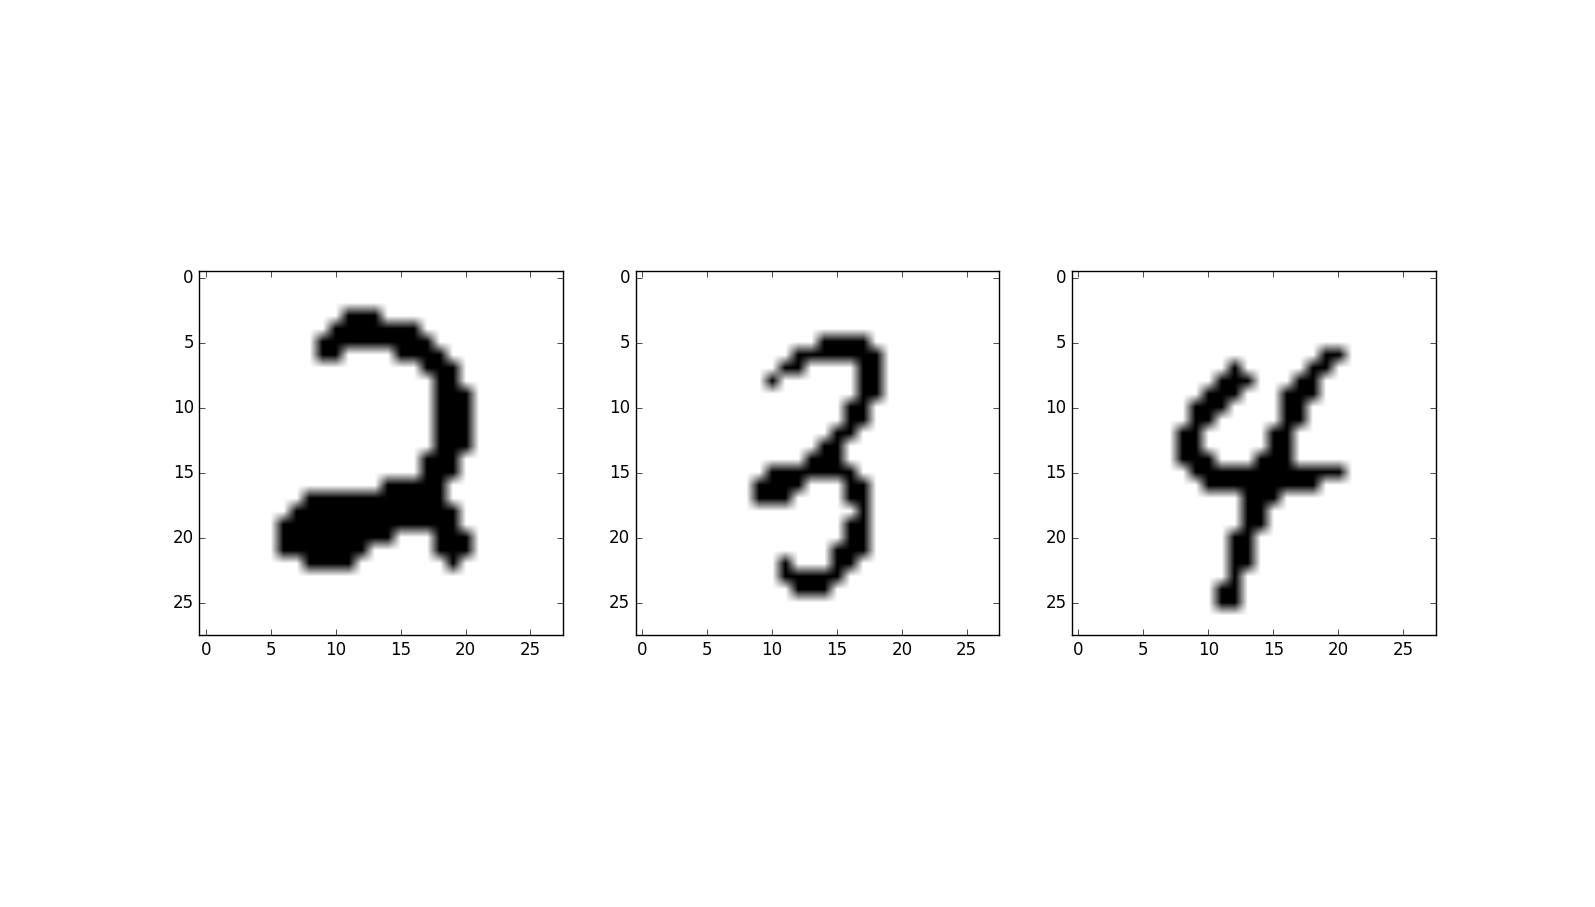
\includegraphics{../Figures/Ex41_examples.png}
	\caption{One sample image of each target class to be trained.}
	\label{fig:41_examples}
\end{figure}
Similar classifications with Mixture models, particularly with Bernoulli distributions have been performed successfully, see e.g. "Bernoulli mixture models for binary images" by Juan and Vidal (2004), so yes, it is possible. Let's maximise our performance!

\subsection{Expectation maximisation for Bernoulli mixture models}\label{sec:42}
The class code has already been appended to the previous section of the document. It is the same class as for the GMMs, with the class variable \texttt{bmm.distrib = 'Bernoulli'} set on initialisation. This then omits a starting value for the covariances, as the responsibilities enter only in terms which can be computed directly (see below).
We can initialise an instance analogously to exercise 3 (see section \ref{sec:43}).

For \texttt{\_do\_mstep} we have replaced formulas (9.24) - (9.26) by (9.59), (9.60), but the implementation stays identical. The loglikelihood can be computed analogously to the sum part of (9.54) (see function \texttt{\_log\_bernoulli\_density}). Thus, algorithmically, the BMM is a simplification of the GMM with another density.

Note, that the images are imported in vector format, to keep the old class structure (other than in part \ref{sec:41}). 
Note also, that we included an numerically small $\epsilon$ (see (9.41), (9.42)) to avoid annihilation of the loglikelihood sum because applying only the logarithm did not work, analogously to the GMM (likely due to numerically different processing than with Matlab).

\subsection{Running the algorithm}\label{sec:43}
After \ref{sec:42} we can now run the algorithm. Let us have a look at how the class means develop (see figure \ref{fig:42_means}).
\begin{figure}[H]
	\centering 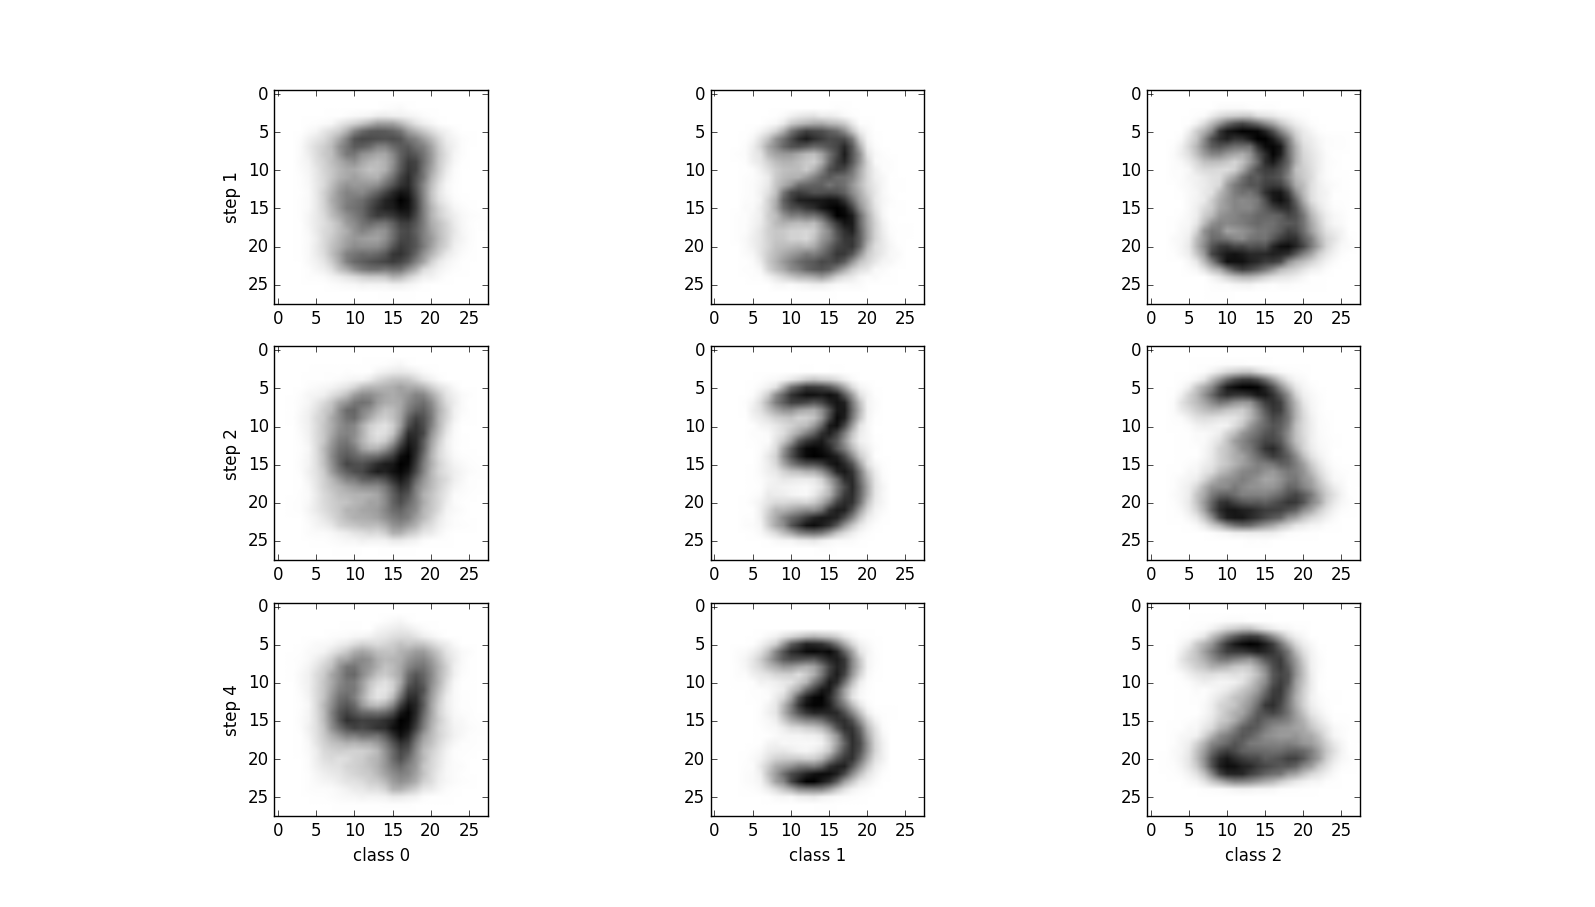
\includegraphics{../Figures/Ex43_means.png}
	\caption{Another example for the rapid progression of EM: after the first steps, hardly any change is visible. At the final step, the images are slightly more smeared.}
	\label{fig:42_means}
\end{figure}
In the first steps, the means appear to be an overlay of the different numbers. As the weights begin to favour one of the classes, the respective digit becomes more distinct. After some steps, the class-digit is clearly readable. From this point on, the mean appears to loose contrast. This can already be interpreted as overfitting.

When comparing the means to cases with $K=4$, we see that in the latter case only the 2 is really pronounced (see figure \ref{fig:43means4}), while the other classes contain mixed features from all digits. This is also the case for $K=2$ (see figure \ref{fig:43means2}), but here 2 and 3 cristallise out and 4 remains missing, while parts of it are still in the left side of the 2.

\begin{figure}[H]
	\centering 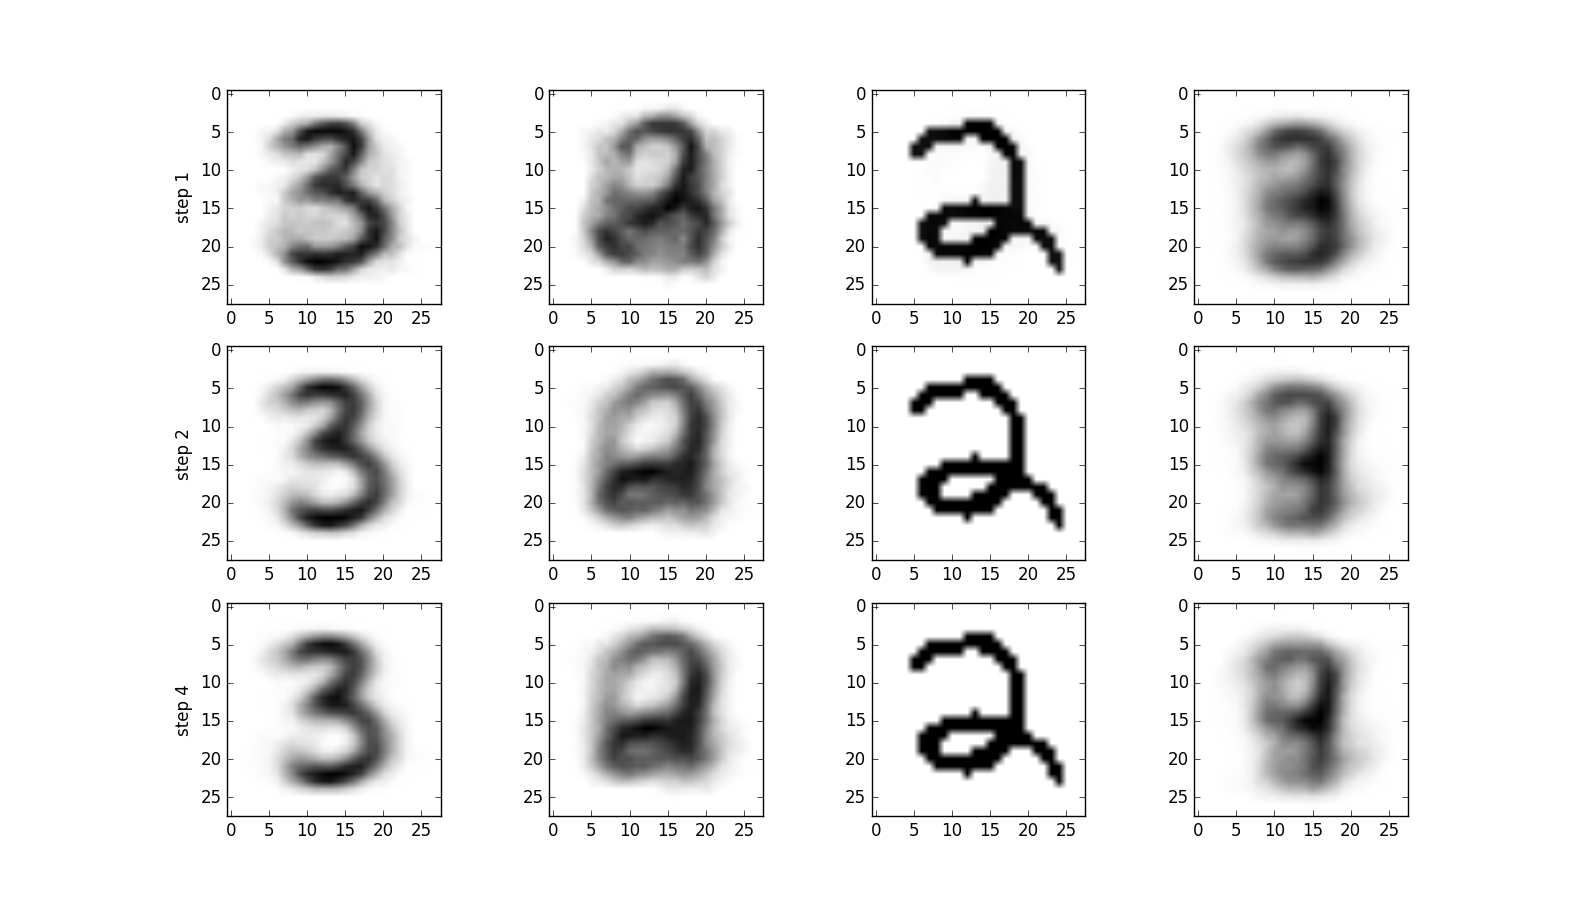
\includegraphics{../Figures/Ex43_means4.png}
	\caption{Class means when forcing $K=4$ components.}
	\label{fig:43means4}
\end{figure}
\begin{figure}[H]
	\centering 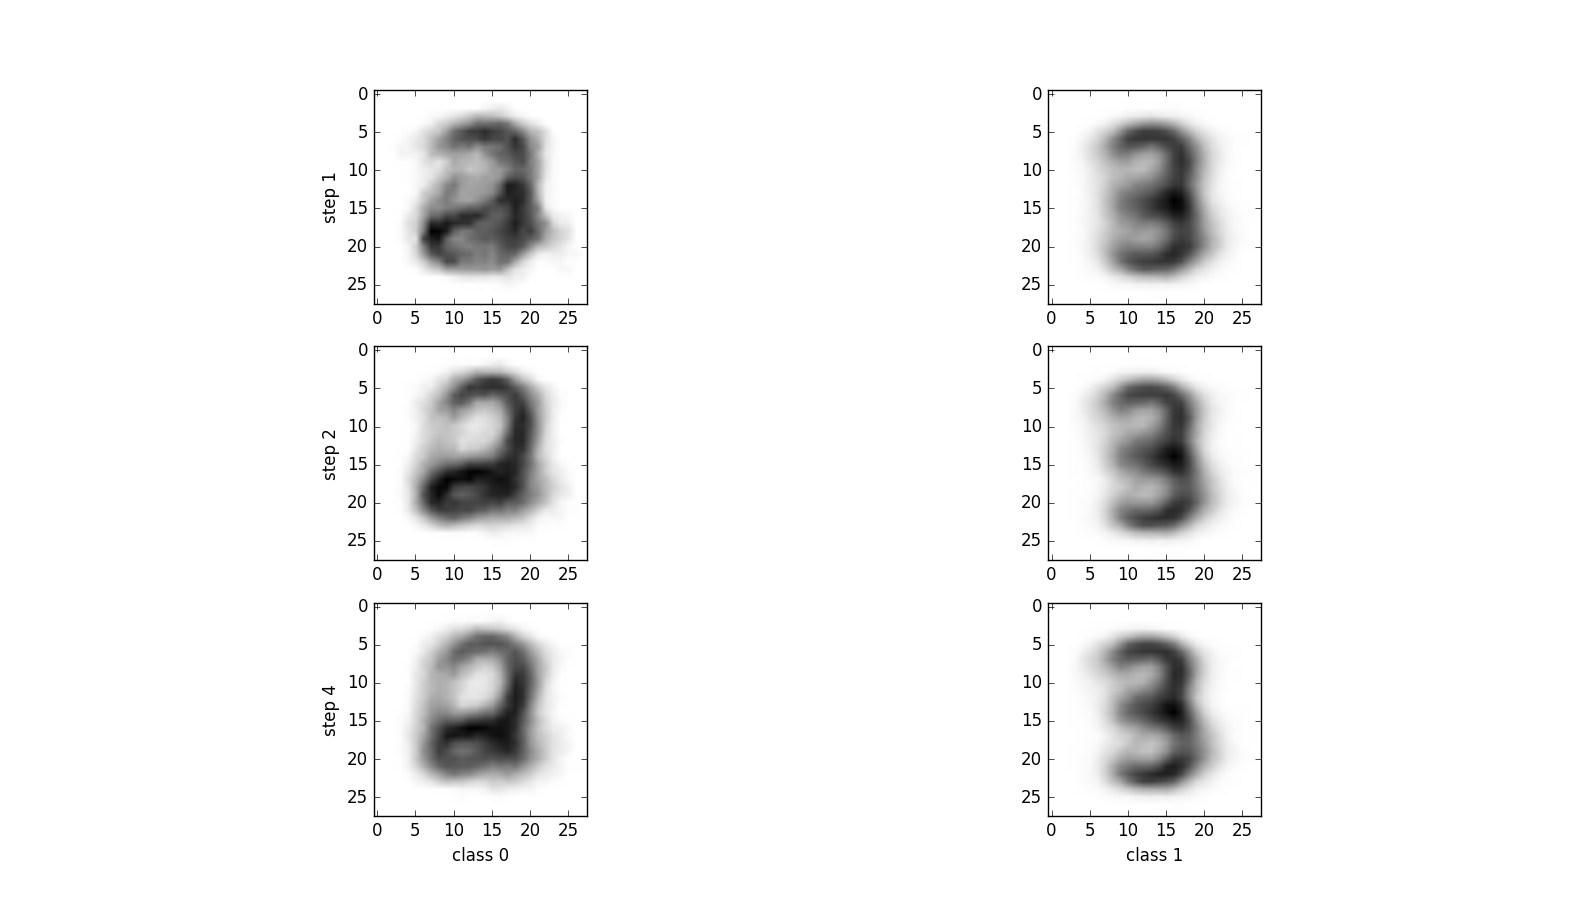
\includegraphics{../Figures/Ex43_means2.png}
	\caption{Class means when forcing $K=4$ components.}
	\label{fig:43means2}
\end{figure}

\subsection{Performance analysis}\label{sec:4.4}
To compare the true labels with the learned ones, we need to permutate our classes to find the right mapping to the MNIST classes.
\begin{verbatim}
    # now let's compare to the ground truth:
    ground_truth = np.fromfile('../Data/a012_labels.dat', dtype=np.int8)
    ground_truth = np.array(ground_truth, dtype=int)
    # we need to permute the labels, to see how many numbers were
    # identified correctly!
    permutation_list = [ ]
    agreement = np.zeros(int(factorial(len(np.unique(labels)))))
    for i, p in enumerate(permutations(np.unique(labels))):
        relabeled = np.zeros_like(labels)
        permutation_list.append(p)
        for j in np.arange(len(np.unique(labels))):
            relabeled[ labels == np.unique(labels)[ j ] ] = p[ j ]
        agreement[ i ] = np.sum(relabeled == ground_truth)
    relabeled = np.zeros_like(labels)
    for j in np.arange(len(np.unique(labels))):
        relabeled[ labels == np.unique(labels)[ j ] ] = permutation_list[
            np.argmax(agreement) ][ j ]
    # how well did we perform?
    performance = np.sum(relabeled == ground_truth)
\end{verbatim}
It turns out, that for our initial instance we already identified 743 labels correctly, which is a performance of 92.875\%.

When changing the number of classes, the performance is obviously reduced. This is reflected in the loglikelihood and the BIC in comparison to the $K=3$-classification (see figures \ref{fig4:3llh3} and \ref{fig4:3llh24}).
\begin{figure}[H]
	\centering 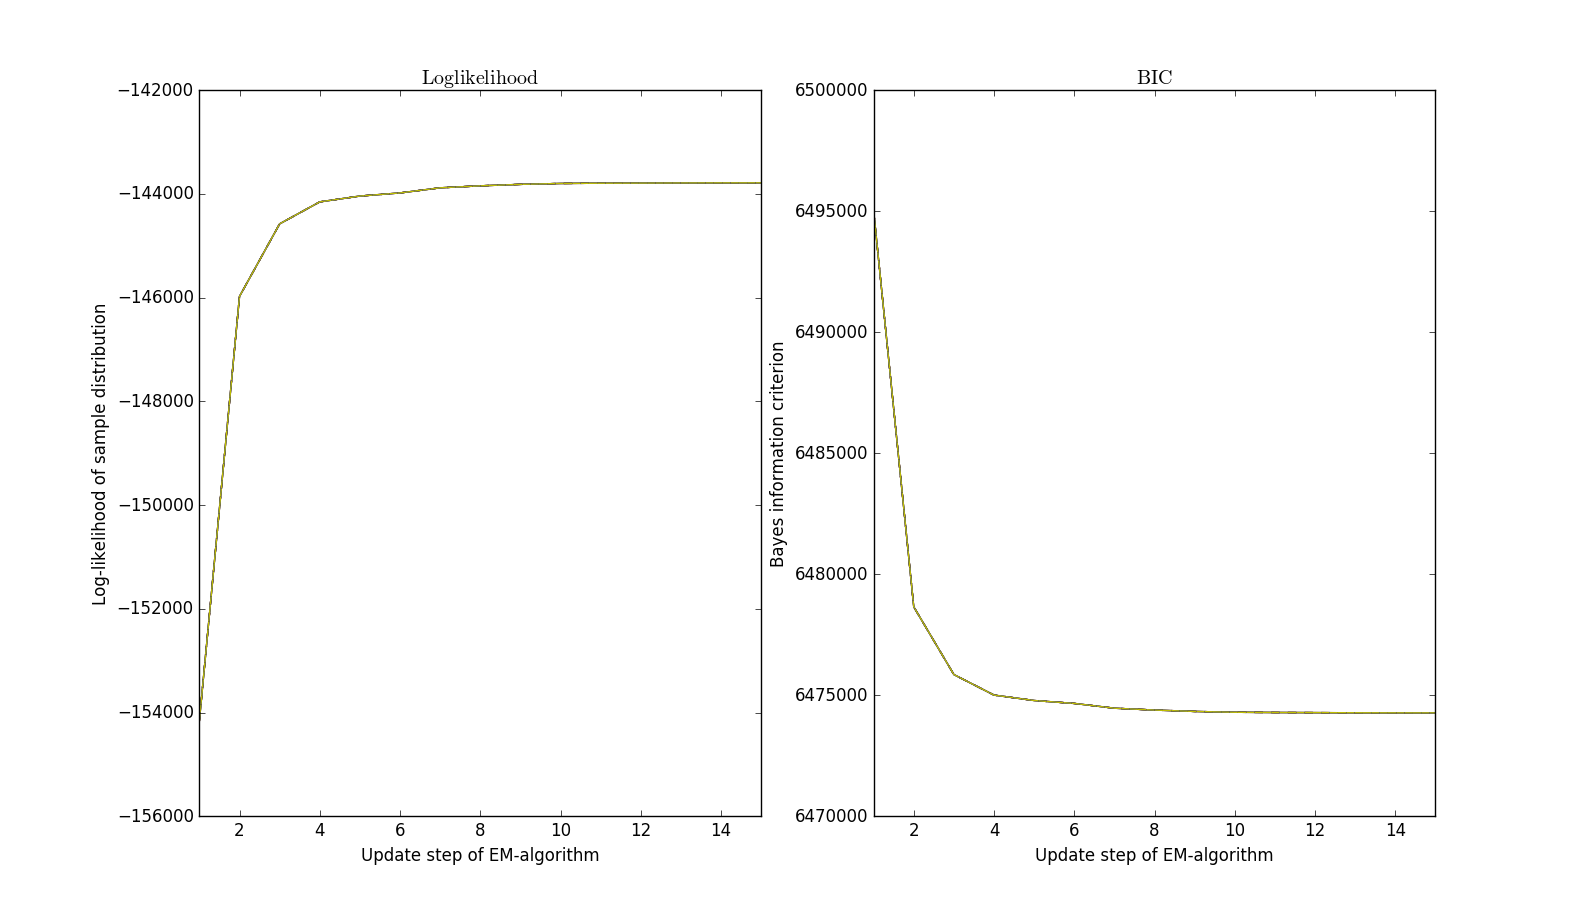
\includegraphics{../Figures/Ex43_llh3.png}
	\caption{The curves for the different initialisations of the $K=3$ model. As in exercise 3, the spanned range is so large (due to rapid convergence) that the plots look virtually identical. When initialising the model with the true means, convergence is slower, because the model "cannot decide" which component to weight in favour of which digit.
	}
	\label{fig4:3llh3}
\end{figure}
\begin{figure}[H]
	\centering 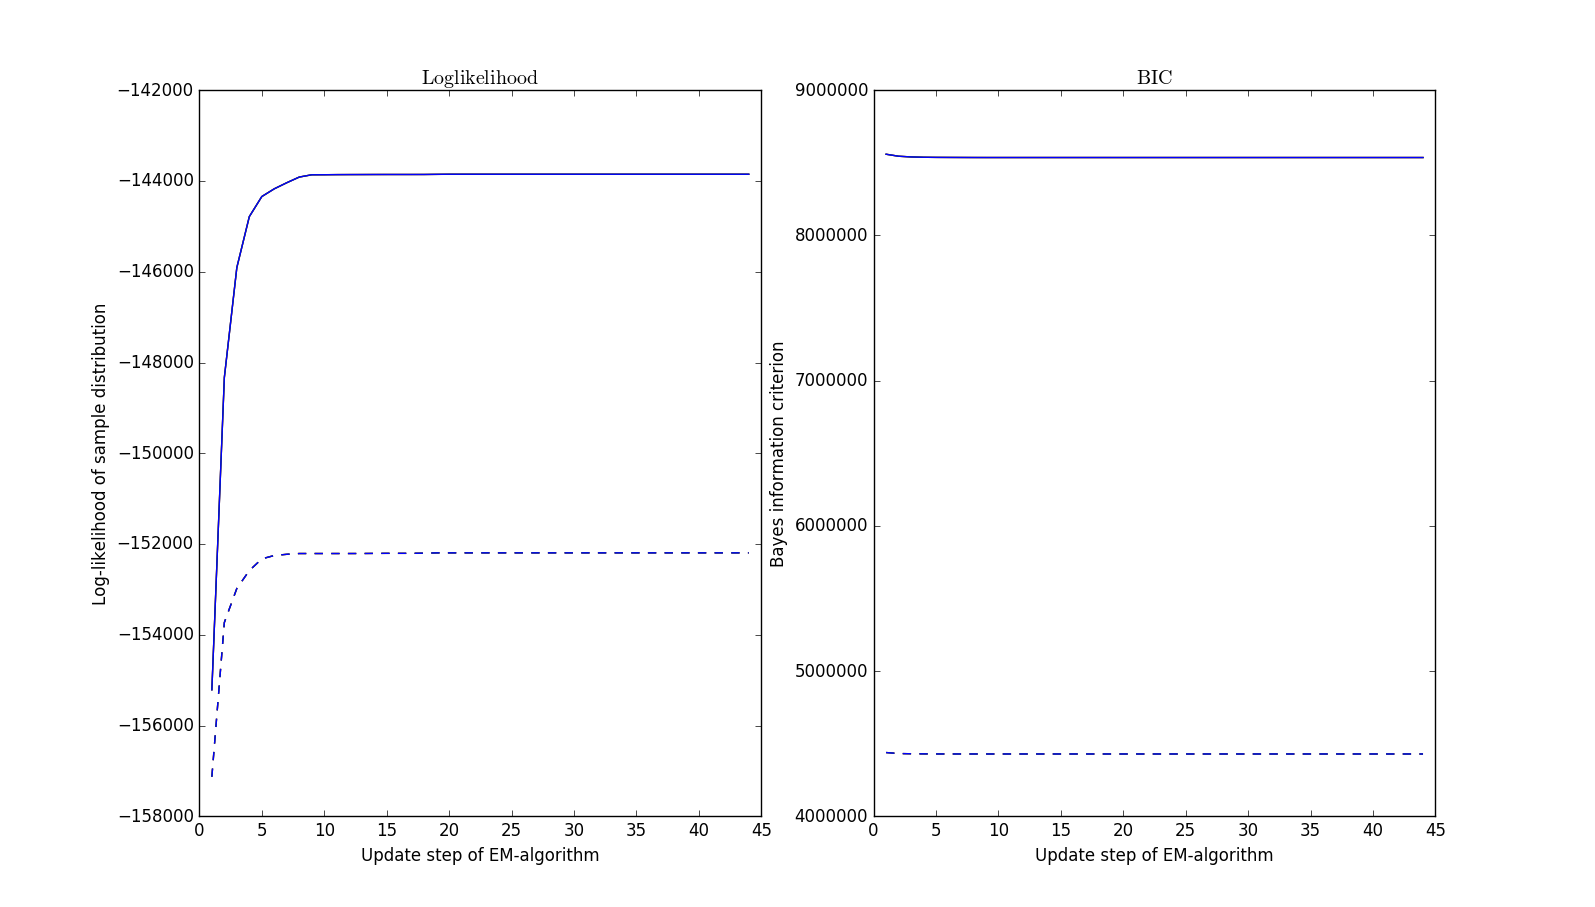
\includegraphics{../Figures/Ex43_llh24.png}
	\caption{The straight lines represent the $K=4$, the dashed lines the $K=2$ model. Obviously, both perform slower and worse in total, than the $K=3$ solutions.}
	\label{fig4:3llh24}
\end{figure}

The differences also become evident when observing the development of class means.

The performance could be improved by splitting the dataset and obtaining a validation set. This would also reduce the overfitting.

\begin{figure}[H]
	\centering 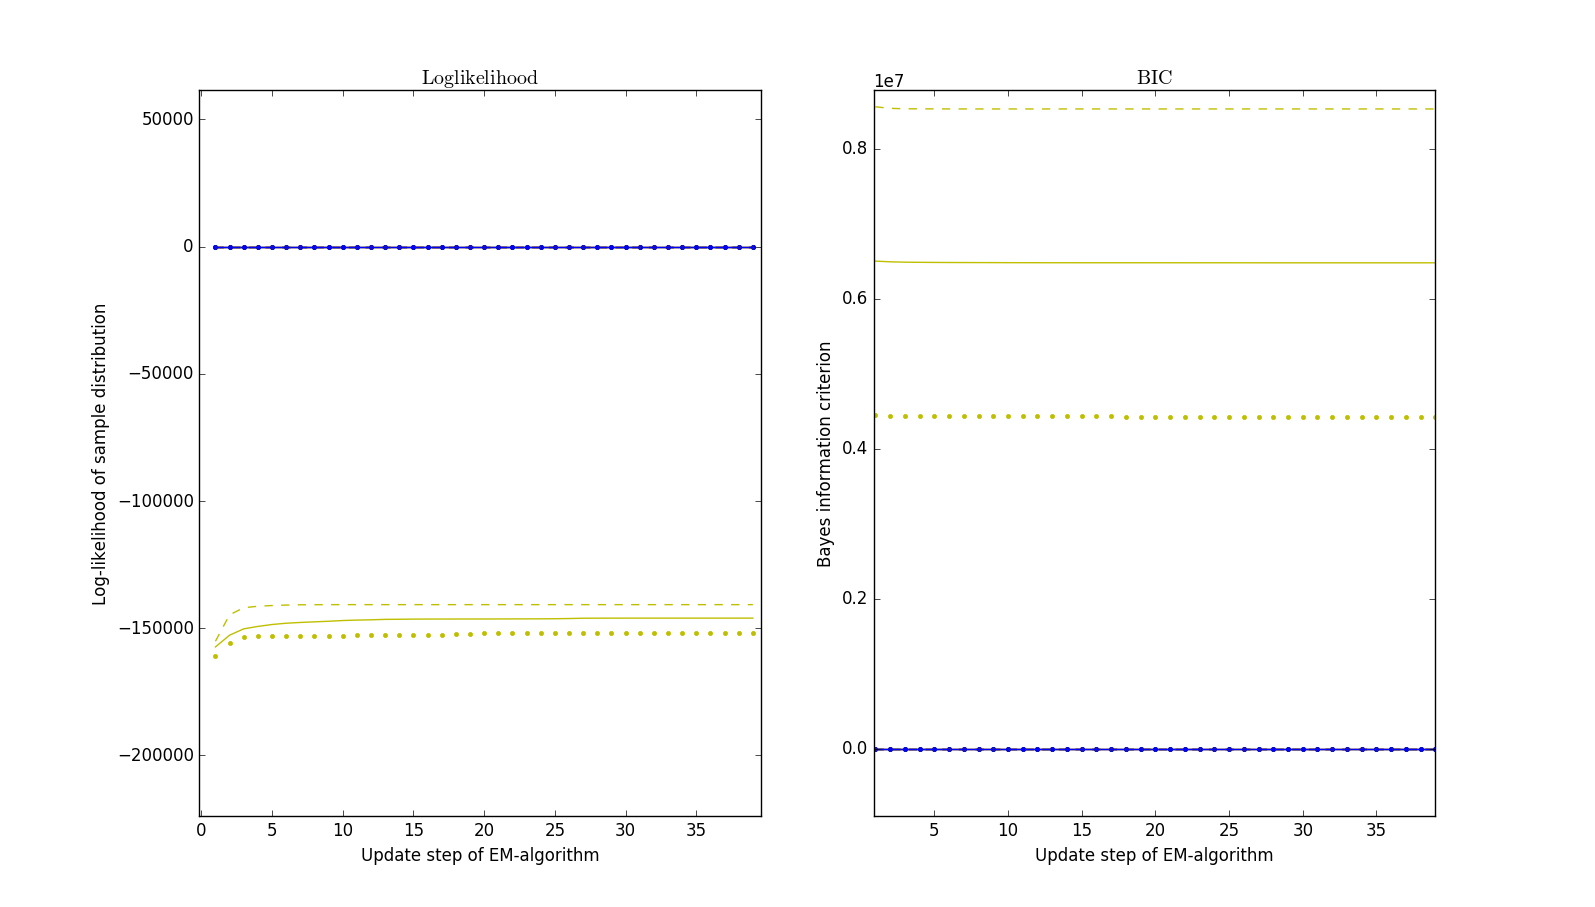
\includegraphics{../Figures/Ex43_llh_all.png}
	\caption{Direct comparison of different component numbers (this looks a bit strange). Straight lines are for 3, dotted for 2 and dashed lines for 4 clusters. The yellow line lies above two other lines, which are generated from different random seeds.}
	\label{fig:43_means_all}
\end{figure}

\subsection{Self-made samples}
This was quite interesting. We started with the following set of handwritten images.
\begin{figure}[H]
	\centering 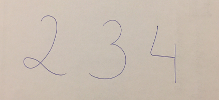
\includegraphics{../Figures/sample_orig.jpg}
	\caption{Handwritten samples.}
	\label{fig:45_handwritten}
\end{figure}
The images had to be separated for individual digits. We then repeatedly applied thresholding and scaled down the image size to obtain $28\times 28$-sized images of grayscales. The result looks like this:
\begin{center}
	\begin{minipage}[t]{0.3\textwidth}
    	\begin{figure}[H]
            
\includegraphics{../Figures/2.png}
    	\end{figure}
	\end{minipage}
	\begin{minipage}[t]{0.3\textwidth}
    	\begin{figure}[H]
            
\includegraphics{../Figures/3.png}
    	\end{figure}
	\end{minipage}
	\begin{minipage}[t]{0.3\textwidth}
    	\begin{figure}[H]
            
\includegraphics{../Figures/4.png}
    	\end{figure}
	\end{minipage}
\end{center}

We then import the images and ask to assign probabilities for the mean classes:
\begin{verbatim}
    import scipy.ndimage as nd
    D = 28
    img1 = nd.imread('../Figures/4.png', flatten=True)/255.
    img2 = nd.imread('../Figures/2.png', flatten=True)/255.
    img3 = nd.imread('../Figures/3.png', flatten=True)/255.
    img1 = np.reshape(1 - np.resize(1 - img1, (28, 28)), D**2)
    img2 = np.reshape(1 - np.resize(1 - img2, (28, 28)), D**2)
    img3 = np.reshape(1 - np.resize(1 - img3, (28, 28)), D**2)
    images = np.vstack((np.vstack((img1, img2)), img3))
    alpha = bmm.predict_proba(images)
    print(alpha)
\end{verbatim}

Considering that there is a permutation in the labelling, the images are assigned the following way:
\begin{verbatim}
[[             inf              inf              inf]
 [  6.64612757e-01   2.14713483e-38   3.35387243e-01]
 [             inf              inf              inf]]
\end{verbatim}
Considering the permutation, the classifier correctly identified the second image as a 2. With the other two images there still seems to be an issue with the log...

\newpage
\section{Code}
\begin{verbatim}
# coding=utf-8
"""
This file contains solutions to Exercise 4 of Assignment 4 of Bert
 Kappen's course "Statistical Machine Learning" 2016/2017.
"""

import numpy as np
from scipy import linalg
import os
import copy
import matplotlib.pyplot as plt
import matplotlib as mpl
import matplotlib.cm as cmx
import mixture_models
from scipy.misc import factorial
from itertools import product
from itertools import permutations

def ground_truth_comparison(labels):
    """Take classification and compare to MNIST labels"""
    # now let's compare to the ground truth:
    ground_truth = np.fromfile('../Data/a012_labels.dat', dtype=np.int8)
    ground_truth = np.array(ground_truth, dtype=int)

    # we need to permute the labels, to see how many numbers were
    # identified correctly!
    permutation_list = [ ]
    agreement = np.zeros(int(factorial(len(np.unique(labels)))))
    for i, p in enumerate(permutations(np.unique(labels))):
        relabeled = np.zeros_like(labels)
        permutation_list.append(p)
        for j in np.arange(len(np.unique(labels))):
            relabeled[ labels == np.unique(labels)[ j ] ] = p[ j ]
        agreement[ i ] = np.sum(relabeled == ground_truth)
    relabeled = np.zeros_like(labels)
    for j in np.arange(len(np.unique(labels))):
        relabeled[ labels == np.unique(labels)[ j ] ] = permutation_list[
            np.argmax(agreement) ][ j ]

    # how well did we perform?
    performance = np.sum(relabeled == ground_truth)
    permutation = permutation_list[ np.argmax(agreement) ]
    return performance, permutation


if __name__ == '__main__':

    ex41 = False  # False just supresses the output, but still loads the data
    ex42 = True
    ex43 = False
    ex442 = False
    ex444 = False
    ex45 = True
    plots1 = False
    plots2 = False
    plots3 = False
    plotnow = False
    the_plot = False
    """
    Exercise 4.1
    """
    # load the image data
    N = 800
    D = 28
    data = np.fromfile('../Data/a012_images.dat', dtype=np.int8)
    data = np.array(data, dtype=int)
    data2 = data.reshape(N, D, D)  # just for visualisation
    data = np.array(data.reshape(N, D**2), dtype=float)
    n_iterations = 45

    if ex41:
        # fig, ax = plt.subplots()
        # for i in np.arange(data2.shape[ 0 ]):
        #     ax.imshow(data2[ i, :, : ].T, cmap='gray_r')
        #     plt.pause(1e-3)
        fig41 = plt.figure()
        ax1 = fig41.add_subplot(131)
        ax1.imshow(data2[ 0, :, : ].T, cmap='gray_r')
        ax2 = fig41.add_subplot(132)
        ax2.imshow(data2[ 1, :, : ].T, cmap='gray_r')
        ax3 = fig41.add_subplot(133)
        ax3.imshow(data2[ 4, :, : ].T, cmap='gray_r')

    """
    Exercise 4.2
    """
    # The class for the BMM algorithm is contained in the mixture models
    if ex42:

        # K = 3 ---------------------------------------------------------
        # set up some stuff for the gaussian mixture models
        n_iterations = 40
        K = 3
        seed = np.random.seed(3)  # shoud be initialised automatically
        # initialisation
        init_means = np.random.random_sample((K, D**2)) * 0.5 + 0.25
        init_weights = np.ones(K, dtype=float) / K

        # Fit a Gaussian mixture with EM using five components
        loglikelihoods = np.zeros(n_iterations)
        criterions = np.zeros(n_iterations)
        convergence_print = False

        # let's initialise the model for a single run.
        bmm = mixture_models.MixtureModel(n_components=K,
                              means_init=init_means,
                              weights_init=init_weights,
                              n_iter=n_iterations,
                              distrib='Bernoulli')
        bmm = bmm.fit(data)
        loglikelihoods = np.sum(bmm.score_samples(data)[ 0 ])
        criterions = bmm.bic(data)
        labels = bmm.score_samples(data)[ 1 ].argmax(axis=1)
        labels += 2

        performance1, permutation1 = ground_truth_comparison(labels)

    """
    Exercise 4.3
    """
    if ex43:
        # --------------------------- K = 3 ------------------------------
        K = 3
        n_randomisations = 4
        n_iterations = 40
        for r in np.arange(n_randomisations):
            print('r = {0}'.format(r))
            seed = np.random.RandomState(r)
            init_means = np.random.random_sample((K, D**2)) * 0.5 + 0.25
            init_weights = np.ones(K, dtype=float) / K
            loglikelihoods = np.zeros((n_iterations, n_randomisations))
            criterions = np.zeros((n_iterations, n_randomisations))
            class_means = np.zeros((n_iterations, K, D**2))
            labels = np.zeros((data.shape[ 0 ], n_iterations))
            convergence_print = False
            for i in np.arange(n_iterations):
                print('iteration = {0}'.format(i))
                bmm = mixture_models.MixtureModel(n_components=K,
                                                  means_init=init_means,
                                                  weights_init=init_weights,
                                                  n_iter=i,
                                                  distrib='Bernoulli',
                                                  random_state=seed)
                bmm = bmm.fit(data)
                # give the class means:
                for k in np.arange(K):
                    class_means[ i, k, : ] = bmm.means_[ k, : ]
                loglikelihoods[ i, r ] = np.sum(bmm.score_samples(data)[ 0 ])
                criterions[ i, r ] = bmm.bic(data)
                # convergence?
                if bmm.converged_ and not convergence_print:
                    print('converged at step {0}'.format(i))
                    convergence_print = True
                labels[ :, r ] = bmm.score_samples(data)[ 1 ].argmax(axis=1)
            labels += 2
                    # break
            if not bmm.converged_:
                print('no convergence in trial {0}'.format(r))

        """
        Exercise 4.4
        """
        # --------------------------- K = 2 ------------------------------
        K = 2
        n_randomisations = 4
        n_iterations = 45
        for r in np.arange(n_randomisations):
            print('r = {0}'.format(r))
            seed = np.random.RandomState(r)
            init_means = np.random.random_sample((K, D**2)) * 0.5 + 0.25
            init_weights = np.ones(K, dtype=float) / K
            loglikelihood2 = np.zeros((n_iterations, n_randomisations))
            criterions2 = np.zeros((n_iterations, n_randomisations))
            class_means2 = np.zeros((n_iterations, n_randomisations, K, D**2))
            labels2 = np.zeros((data.shape[ 0 ], n_randomisations))
            convergence_print = False
            for i in np.arange(n_iterations):
                print('iteration = {0}'.format(i))
                bmm2 = mixture_models.MixtureModel(n_components=K,
                                                  means_init=init_means,
                                                  weights_init=init_weights,
                                                  n_iter=i,
                                                  distrib='Bernoulli',
                                                  random_state=seed)
                bmm2 = bmm2.fit(data)
                # give the class means:
                for k in np.arange(K):
                    class_means2[ i, r, k, : ] = bmm2.means_[ k, : ]
                loglikelihood2[ i, r ] = np.sum(bmm2.score_samples(data)[ 0 ])
                criterions2[ i, r ] = bmm2.bic(data)
                # convergence?
                if bmm2.converged_ and not convergence_print:
                    print('converged at step {0}'.format(i))
                    convergence_print = True
                labels2[ :, r ] = bmm2.score_samples(data)[ 1 ].argmax(
                        axis=1)
            labels2 += 2
                    # break
            if not bmm2.converged_:
                print('no convergence in trial {0}'.format(r))

        # --------------------------- K = 4 ------------------------------
        K = 4
        n_randomisations = 4
        n_iterations = 45
        for r in np.arange(n_randomisations):
            print('r = {0}'.format(r))
            seed = np.random.RandomState(r)
            init_means = np.random.random_sample((K, D**2)) * 0.5 + 0.25
            init_weights = np.ones(K, dtype=float) / K
            loglikelihoods4 = np.zeros((n_iterations, n_randomisations))
            criterions4 = np.zeros((n_iterations, n_randomisations))
            class_means4 = np.zeros((n_iterations, n_randomisations, K, D**2))
            labels4 = np.zeros((data.shape[ 0 ], n_randomisations))
            convergence_print = False
            for i in np.arange(n_iterations):
                print('iteration = {0}'.format(i))
                bmm4 = mixture_models.MixtureModel(n_components=K,
                                                  means_init=init_means,
                                                  weights_init=init_weights,
                                                  n_iter=i,
                                                  distrib='Bernoulli',
                                                  random_state=seed)
                bmm4 = bmm4.fit(data)
                # give the class means:
                for k in np.arange(K):
                    class_means4[ i, r, k, : ] = bmm4.means_[ k, : ]
                loglikelihoods4[ i, r ] = np.sum(bmm4.score_samples(data)[ 0 ])
                criterions4[ i, r ] = bmm4.bic(data)
                # convergence?
                if bmm4.converged_ and not convergence_print:
                    print('converged at step {0}'.format(i))
                    convergence_print = True
                labels4[ :, r ] = bmm4.score_samples(data)[ 1 ].argmax(
                        axis=1)
                    # break
            labels4 += 2
            if not bmm4.converged_:
                print('no convergence in trial {0}'.format(r))

    if plots1:
        fig431 = plt.figure()
        ax1 = fig431.add_subplot(331)
        ax1.imshow(class_means[ 1, 0, 0, : ].reshape(D, D).T,
                   cmap='gray_r')
        ax1.set_ylabel('step 1', size=12)
        ax2 = fig431.add_subplot(332)
        ax2.imshow(class_means[ 1, 0, 1, : ].reshape(D, D).T,
                   cmap='gray_r')
        ax3 = fig431.add_subplot(333)
        ax3.imshow(class_means[ 1, 0, 2, : ].reshape(D, D).T,
                   cmap='gray_r')
        ax4 = fig431.add_subplot(334)
        ax4.imshow(class_means[ 2, 0, 0, : ].reshape(D, D).T,
                   cmap='gray_r')
        ax4.set_ylabel('step 2', size=12)
        ax5 = fig431.add_subplot(335)
        ax5.imshow(class_means[ 2, 0, 1, : ].reshape(D, D).T,
                   cmap='gray_r')
        ax6 = fig431.add_subplot(336)
        ax6.imshow(class_means[ 2, 0, 2, : ].reshape(D, D).T,
                   cmap='gray_r')
        ax7 = fig431.add_subplot(337)
        ax7.imshow(class_means[ 4, 0, 0, : ].reshape(D, D).T,
                   cmap='gray_r')
        ax7.set_ylabel('step 4', size=12)
        ax7.set_xlabel('class 0', size=12)
        ax8 = fig431.add_subplot(338)
        ax8.imshow(class_means[ 4, 0, 1, : ].reshape(D, D).T,
                   cmap='gray_r')
        ax8.set_xlabel('class 1', size=12)
        ax9 = fig431.add_subplot(339)
        ax9.imshow(class_means[ 4, 0, 2, : ].reshape(D, D).T,
                   cmap='gray_r')
        ax9.set_xlabel('class 2', size=12)

    if plots2:
        fig331 = plt.figure()
        ax1 = fig331.add_subplot(121)
        ax1.plot(np.arange(1, n_iterations), loglikelihoods[ 1:, 0 ], 'b',
                 )
        ax1.set_xlabel('Update step of EM-algorithm')
        ax1.set_ylabel('Log-likelihood of sample distribution')
        ax1.set_xlim([ 1, 20 ])
        ax1.set_ylim([ -170000, -160000 ])
        plt.title(r'$\mathrm{Loglikelihood}$')
        ax2 = fig331.add_subplot(122)
        ax2.plot(np.arange(1, n_iterations), criterions[ 1:, 0 ], 'b',
                 )
        ax2.set_xlim([ 1, 20 ])
        ax2.set_xlabel('Update step of EM-algorithm')
        ax2.set_ylabel('Bayes information criterion')
        plt.title(r'$\mathrm{BIC}$')

    if ex45:
        # import
        import scipy.ndimage as nd
        D = 28
        img1 = nd.imread('../Figures/4.png', flatten=True)/256.
        img2 = nd.imread('../Figures/2.png', flatten=True)/256.
        img3 = nd.imread('../Figures/3.png', flatten=True)/256.
        img1 = np.reshape(np.resize(1 - img1, (28, 28)), D**2)
        img2 = np.reshape(np.resize(1 - img2, (28, 28)), D**2)
        img3 = np.reshape(np.resize(1 - img3, (28, 28)), D**2)
        images = np.vstack((np.vstack((img1, img2)), img3))
        alpha = bmm.predict_proba(images)
        print(alpha)

    if plots3:
        fig441 = plt.figure()
        ax1 = fig441.add_subplot(121)
        ax1.plot(np.arange(1, n_iterations), loglikelihoods4[ 1:, 0 ], 'r',
                 np.arange(1, n_iterations), loglikelihoods4[ 1:, 1 ], 'g',
                 np.arange(1, n_iterations), loglikelihoods4[ 1:, 2 ], 'b',
                 # np.arange(1, n_iterations), loglikelihoods4[ 1:, 3 ], 'y',
                 np.arange(1, n_iterations), loglikelihood2[ 1:, 0 ], 'r--',
                 np.arange(1, n_iterations), loglikelihood2[ 1:, 1 ], 'g--',
                 np.arange(1, n_iterations), loglikelihood2[ 1:, 2 ], 'b--',
                 # np.arange(1, n_iterations), loglikelihood2[ 1:, 3 ], 'y--'
                 )
        ax1.set_xlabel('Update step of EM-algorithm')
        ax1.set_ylabel('Log-likelihood of sample distribution')
        plt.title(r'$\mathrm{Loglikelihood}$')
        ax2 = fig441.add_subplot(122)
        ax2.plot(np.arange(1, n_iterations), criterions4[ 1:, 0 ], 'r',
                 np.arange(1, n_iterations), criterions4[ 1:, 1 ], 'g',
                 np.arange(1, n_iterations), criterions4[ 1:, 2 ], 'b',
                 # np.arange(1, n_iterations), criterions4[ 1:, 3 ], 'y',
                 np.arange(1, n_iterations), criterions2[ 1:, 0 ], 'r--',
                 np.arange(1, n_iterations), criterions2[ 1:, 1 ], 'g--',
                 np.arange(1, n_iterations), criterions2[ 1:, 2 ], 'b--',
                 # np.arange(1, n_iterations), criterions2[ 1:, 3 ], 'y--'
                 )
        ax2.set_xlabel('Update step of EM-algorithm')
        ax2.set_ylabel('Bayes information criterion')
        plt.title(r'$\mathrm{BIC}$')

    if the_plot:
        n_iterations = 40
        fig442 = plt.figure()
        ax1 = fig442.add_subplot(121)
        ax1.plot(
                np.arange(1, n_iterations), loglikelihoods[ 1:n_iterations, 0 ], 'r',
                np.arange(1, n_iterations), loglikelihoods[ 1:n_iterations, 1 ], 'g',
                np.arange(1, n_iterations), loglikelihoods[ 1:n_iterations, 2 ], 'b',
                np.arange(1, n_iterations), loglikelihoods[ 1:n_iterations, 3 ], 'y',
                np.arange(1, n_iterations), loglikelihood2[ 1:n_iterations, 0 ], 'r.',
                np.arange(1, n_iterations), loglikelihood2[ 1:n_iterations, 1 ], 'g.',
                np.arange(1, n_iterations), loglikelihood2[ 1:n_iterations, 2 ], 'b.',
                np.arange(1, n_iterations), loglikelihood2[ 1:n_iterations, 3 ], 'y.',
                np.arange(1, n_iterations), loglikelihoods4[ 1:n_iterations, 0 ], 'r--',
                np.arange(1, n_iterations), loglikelihoods4[ 1:n_iterations, 1 ], 'g--',
                np.arange(1, n_iterations), loglikelihoods4[ 1:n_iterations, 2 ], 'b--',
                np.arange(1, n_iterations), loglikelihoods4[ 1:n_iterations, 3 ], 'y--'
                )
        ax1.set_xlim([1, 15])
        ax1.set_xlabel('Update step of EM-algorithm')
        ax1.set_ylabel('Log-likelihood of sample distribution')
        plt.title(r'$\mathrm{Loglikelihood}$')
        ax2 = fig442.add_subplot(122)
        ax2.plot(
                np.arange(1, n_iterations), criterions[ 1:n_iterations, 0 ], 'r',
                np.arange(1, n_iterations), criterions[ 1:n_iterations, 1 ], 'g',
                np.arange(1, n_iterations), criterions[ 1:n_iterations, 2 ], 'b',
                np.arange(1, n_iterations), criterions[ 1:n_iterations, 3 ], 'y',
                np.arange(1, n_iterations), criterions2[ 1:n_iterations, 0 ], 'r.',
                np.arange(1, n_iterations), criterions2[ 1:n_iterations, 1 ], 'g.',
                np.arange(1, n_iterations), criterions2[ 1:n_iterations, 2 ], 'b.',
                np.arange(1, n_iterations), criterions2[ 1:n_iterations, 3 ], 'y.',
                np.arange(1, n_iterations), criterions4[ 1:n_iterations, 0 ], 'r--',
                np.arange(1, n_iterations), criterions4[ 1:n_iterations, 1 ], 'g--',
                np.arange(1, n_iterations), criterions4[ 1:n_iterations, 2 ], 'b--',
                np.arange(1, n_iterations), criterions4[ 1:n_iterations, 3 ], 'y--'
                )
        ax2.set_xlim([ 1, 15 ])
        ax2.set_xlabel('Update step of EM-algorithm')
        ax2.set_ylabel('Bayes information criterion')
        plt.title(r'$\mathrm{BIC}$')


# ----------------------------------------------------------------------------
    if plotnow:
        fig443 = plt.figure()
        ax1 = fig443.add_subplot(341)
        ax1.imshow(class_means[ 1, 0, : ].reshape(D, D).T, cmap='gray_r')
        ax1.set_ylabel('step 1', size=12)
        ax2 = fig443.add_subplot(342)
        ax2.imshow(class_means[ 1, 1, : ].reshape(D, D).T, cmap='gray_r')
        ax3 = fig443.add_subplot(343)
        ax3.imshow(class_means[ 1, 2, : ].reshape(D, D).T, cmap='gray_r')
        ax4 = fig443.add_subplot(344)
        ax4.imshow(class_means[ 1, 3, : ].reshape(D, D).T, cmap='gray_r')
        ax5 = fig443.add_subplot(345)
        ax5.imshow(class_means[ 2, 0, : ].reshape(D, D).T, cmap='gray_r')
        ax5.set_ylabel('step 2', size=12)
        ax6 = fig443.add_subplot(346)
        ax6.imshow(class_means[ 2, 1, : ].reshape(D, D).T, cmap='gray_r')
        ax7 = fig443.add_subplot(347)
        ax7.imshow(class_means[ 2, 2, : ].reshape(D, D).T, cmap='gray_r')
        ax8 = fig443.add_subplot(348)
        ax8.imshow(class_means[ 2, 3, : ].reshape(D, D).T, cmap='gray_r')
        ax9 = fig443.add_subplot(349)
        ax9.imshow(class_means[ 4, 0, : ].reshape(D, D).T, cmap='gray_r')
        ax9.set_ylabel('step 4', size=12)
        ax10 = fig443.add_subplot(3,4,10)
        ax10.imshow(class_means[ 4, 1, : ].reshape(D, D).T, cmap='gray_r')
        ax11 = fig443.add_subplot(3,4,11)
        ax11.imshow(class_means[ 4, 2, : ].reshape(D, D).T, cmap='gray_r')
        ax12 = fig443.add_subplot(3,4,12)
        ax12.imshow(class_means[ 4, 3, : ].reshape(D, D).T, cmap='gray_r')

        fig444 = plt.figure()
        ax1 = fig444.add_subplot(321)
        ax1.imshow(class_means[ 1, 0, : ].reshape(D, D).T, cmap='gray_r')
        ax1.set_ylabel('step 1', size=12)
        ax2 = fig444.add_subplot(322)
        ax2.imshow(class_means[ 1, 1, : ].reshape(D, D).T, cmap='gray_r')
        ax3 = fig444.add_subplot(323)
        ax3.imshow(class_means[ 2, 0, : ].reshape(D, D).T, cmap='gray_r')
        ax3.set_ylabel('step 2', size=12)
        ax4 = fig444.add_subplot(324)
        ax4.imshow(class_means[ 2, 1, : ].reshape(D, D).T, cmap='gray_r')
        ax5 = fig444.add_subplot(325)
        ax5.imshow(class_means[ 4, 0, : ].reshape(D, D).T, cmap='gray_r')
        ax5.set_ylabel('step 4', size=12)
        ax5.set_xlabel('class 0', size=12)
        ax6 = fig444.add_subplot(326)
        ax6.imshow(class_means[ 4, 1, : ].reshape(D, D).T, cmap='gray_r')
        ax6.set_xlabel('class 1', size=12)

        plt.show()
\end{verbatim}
    \end{document}
